\documentclass{endm}
\usepackage{endmmacro}
\usepackage{graphicx}
\usepackage[spanish]{babel}


% The following is enclosed to allow easy detection of differences in
% ascii coding.
% Upper-case    A B C D E F G H I J K L M N O P Q R S T U V W X Y Z
% Lower-case    a b c d e f g h i j k l m n o p q r s t u v w x y z
% Digits        0 1 2 3 4 5 6 7 8 9
% Exclamation   !           Double quote "          Hash (number) #
% Dollar        $           Percent      %          Ampersand     &
% Acute accent  '           Left paren   (          Right paren   )
% Asterisk      *           Plus         +          Comma         ,
% Minus         -           Point        .          Solidus       /
% Colon         :           Semicolon    ;          Less than     <
% Equals        =           Greater than >          Question mark ?
% At            @           Left bracket [          Backslash     \
% Right bracket ]           Circumflex   ^          Underscore    _
% Grave accent  `           Left brace   {          Vertical bar  |
% Right brace   }           Tilde        ~

\newcommand{\Nat}{{\mathbb N}}
\newcommand{\Real}{{\mathbb R}}
\def\lastname{Please list your Lastname here}

\begin{document}

% DO NOT REMOVE: Creates space for Elsevier logo, ScienceDirect logo
% and ENDM logo
\begin{verbatim}\end{verbatim}\vspace{2.5cm}

\begin{frontmatter}

\title{Hoy te convert\'is en (Junior) Data Scientist}

%\author{My Name\thanksref{ALL}\thanksref{myemail}}
\author{Ricardo Colombo}
\author{Diego Santos}
\author{Erik Machicado}
%\address{My Department\\ My University\\ My City, My Country}
\address{Departamento de Computaci\'on\\ Universidad de Buenos Aires\\ C.A.B.A, Argentina}

% \author{My Co-author\thanksref{coemail}}
% \address{My Co-author's Department\\ My Co-author's University\\
%    My Co-author's City, My Co-author's Country} \thanks[ALL]{Thanks
%    to everyone who should be thanked} \thanks[myemail]{Email:
%    \href{mailto:myuserid@mydept.myinst.myedu} {\texttt{\normalshape
%    myuserid@mydept.myinst.myedu}}} \thanks[coemail]{Email:
%    \href{mailto:couserid@codept.coinst.coedu} {\texttt{\normalshape
%    couserid@codept.coinst.coedu}}}

% \begin{abstract}
% This is a short example to show the basics of using the ENDM style
% macro files. Ample examples of how files should look may be found
% among the published volumes of the series at the ENDM home page
% ({\texttt{http://www.elsevier.com/locate/endm}})
% \end{abstract}

\begin{abstract}
El trabajo consiste en aplicar t\'ecnicas de M\'etodos num\'ericos y 
Data Science, en particular Regresiones Lineales y Cuadrados M\'inimos, 
a un gran conjunto de datos reales, buscando identificar modelos 
capaces de predecir comportamientos.
\end{abstract}

\begin{keyword}
Data Science, KPIs, Cuadrados Minimos Lineales (CML)
\end{keyword}

\end{frontmatter}


\section{Introducci\'on}\label{intro}

%Contendrá una breve explicación de la base teórica que fundamenta los métodos involucrados en el trabajo, junto con los métodos mismos. No deben incluirse demostraciones de propiedades ni teoremas, ejemplos innecesarios, ni definiciones elementales (como por ejemplo la de matriz simétrica). En vez de definiciones básicas es conveniente citar ejemplos de bibliografía adecuada. Una cita vale más que mil palabras

En la competitiva industria aeron\'autica la eficiencia de los procesos es vital para mantener la calidad del servicio. Cumplir con el servicio no es algo que solo dependa de la empresa que se contrata, ya que a\~no a a\~no la cantidad de vuelos se multipilica y muchas veces existen variables externas que terminen afectando la puntualidad y calidad del servicio. Por eso es importante contar con m\'etricas que analizen los eventos pasados buscando patrones e intentar prevenirlos o desminuir su impacto en el futuro. Estos indicadores son denominados \textit{Key Performance Indicators} (KPIs).

En este trabajo estudiaremos factores que influyen en la organizaci\'on de las salidas de vuelos para un aeropuerto en particular. Como se mencion\'o anteriormente, estad\'isticamente todos los a\~nos se registran mas vuelos para cualquier aeropuerto, esto requiere una sincronizaci\'on precisa de los tiempos que ocupa un avi\'on dentro del aeropuerto esperando para partir.

Nuestro primer eje de estudio se centra en los factores estacionales que influyen en un vuelo salga en tiempo y forma, es decir estudiaremos la cantidad de retrasos en partidas para un aeropuerto particular, con el objetivo de detectar las estaciones anuales donde el clima pueda afectar el funcionamiento del aeropuerto.

Nuestro segundo eje de estudio es la evoluci\'on en la cantidad de tr\'afico \'aereo de un aeropuerto, y como la cuota de \textit{market share} se fue concentrando con el correr del tiempo sobre las empresas l\'ideres del segmento. Lo interesante de esta evaluaci\'on es esperamos poder proyectar el crecimiento de tr\'afico sobre el aeropuerto a fin de poder satisfacer la creciente demanda.

Para la realización del trabajo analizaremos un set de datos reales correspondientes a vuelos realizados en Estados Unidos durante el per\'iodo 2004 - 2008 dado a que no habia datos para años anteriores a 2004 en relacion a nuestras KPI's y la busqueda de encontrar una relacion entre ambos ejes de estudio.

Luego relacionaremos los ejes de estudio para estudiar si es posible predecir temporadas de mayor retraso, esperando que sea de utilidad en la programaci\'on de los nuevos vuelos que se incorporán al mercado.


%breve explicacion de metodo
\paragraph{Metodo de Minimos Cuadrados}

Minimos cuadrados es una t\'ecnica de an\'alisis num\'erico, en la que, dados un conjunto de pares ordenados intenta encontrar la funci\'on que mejor aproxime a los datos de acuerdo con el criterio de Error cuadr\'atico medio. En su forma m\'as simple, intenta minimizar la suma de los cuadrados de las diferencias entre los puntos generados por la funci\'on de aproximaci\'on y los que corresponden a los datos. CML es el caso en el que se usa a las rectas para la aproximaci\'on osea $y = ax + b$, adem\'as la generalizaci\'on del m\'etodo propone encontrar la funci\'on que mejor aproxima de la forma $y = a_1f_1(x) + \dots + a_Kf_K(x)$ y que no es necesario que las funciones $f$ sean lineales pero si que $y$ sea una combinaci\'on lineal de ellas. Para mas informacion consultar  \cite{bf} (seccion 8.1)

\section{Desarrollo}
	%Deben explicarse los métodos numéricos que utilizaron y su aplicación al problema concreto involucrado en el trabajo práctico. Se deben mencionar los pasos que siguieron para implementar los algoritmos, las dificultades que fueron encontrando y la descripción de cómo las fueron resolviendo. Explicar también cómo fueron planteadas y realizadas las mediciones experimentales. Los ensayos fallidos, hipótesis y conjeturas equivocadas, experimentos y métodos malogrados deben figurar en esta sección, con una breve explicación de los motivos de estas fallas (en caso de ser conocidas).

Para la simplificaci\'on del problema y dado a que es replicable en otros aeropuertos optamos por centrarnos en el aeropueto \textit{JFK} debido a que hoy d\'ia es uno de los aeropuertos que m\'as movimiento presenta por la importancia que presenta la ciudad donde est\'a ubicado y sabiendo que tiene estaciones invernales marcadas a fines de a\˜no que afectar\'ian los vuelos ayudandonos en nuestro analisis.  Como primer eje estudiaremos la cantidad de demoras que se producen por condiciones clim\'aticas. Tomando como definici\'on de demora, un vuelo que sale al menos 15 minutos despues de su horario programado ademas de que este tenga una demora debido al clima. El objetivo de este caso es identificar temporadas c\'iciclas donde las condiciones clim\'aticas afectan el comportamiento normal del aeropuerto. Luego como segundo eje estudiaremos la evoluci\'on de la cantidad de vuelos de ese aeropuerto,entre dos de las empresas mas reconocidas mundialemente \textit{Delta} y \textit{United Airlines} y con mayor presencia de vuelos viendo su evoluci\'on a traves de los a\~nos.

Para finalizar intentaremos probar si hay alguna relaci\'on entre el crecimiento de los vuelos y la cantidad de demoras estacionales generadas por el clima, una primera hip\'otesis que tenemos es que al aumentar el trafico aéreo la demora por clima deber\'ia aumentar pese a que no tienen relaci\'on directa creemos que cuando se demora un avi\'on por clima arrastra esta demora a los dem\'as.

Para la realizaci\'on del estudio implementamos una serie de algoritmos utilizando el lenguaje \textit{Python}. En la primer etapa procesamos el data set inicial filtrando los registros que nos interesa estudiar y los agrupamos por mes. Luego para entrenar nuestra soluci\'on propuesta tomamos un subconjunto de meses de los datos conocidos hasta encontrar el que nos de la mejor aproximacion, ejecutamos el proceso para una cantidad \textit{n} tambi\'en buscando la mejor combinacion con los meses elegidos y validamos los resultados obtenidos utilizando la t\'ecnica de \textit{Coss-Validation}. Qued\'andonos con los que min\'imizen el error. Para evitar caer en el conocido overfitting elegiremos distintos subconjuntos del training para hallar los coeficientes de la aproximacion lineal, para ambos entrenamientos usamos el periodo 2004-2007 para entrenamiento y test,  luego realizamos una aproximacion sobre el a\˜n 2008 y lo comparamos con los resultados reales.

Luego el siguiente paso es ver como con los datos entrenados nuestras funciones que tan bien aproximan al valor real e intentar predecir el comportamiento futuro.


\section{Demoras Clim\'aticas}

Como mencionamos anteriormente el aeropuerto estudiado tiene temporadas marcadas y estas se puede observar en el grafico siguiente en forma de picos en el medio de cada a\˜no y en a finales del a\˜no donde tienen nevadas, ademas que se ven esos 2 picos se ven dos caidas en las demoras entre medio marcnado las otras estaciones.

\begin{center}
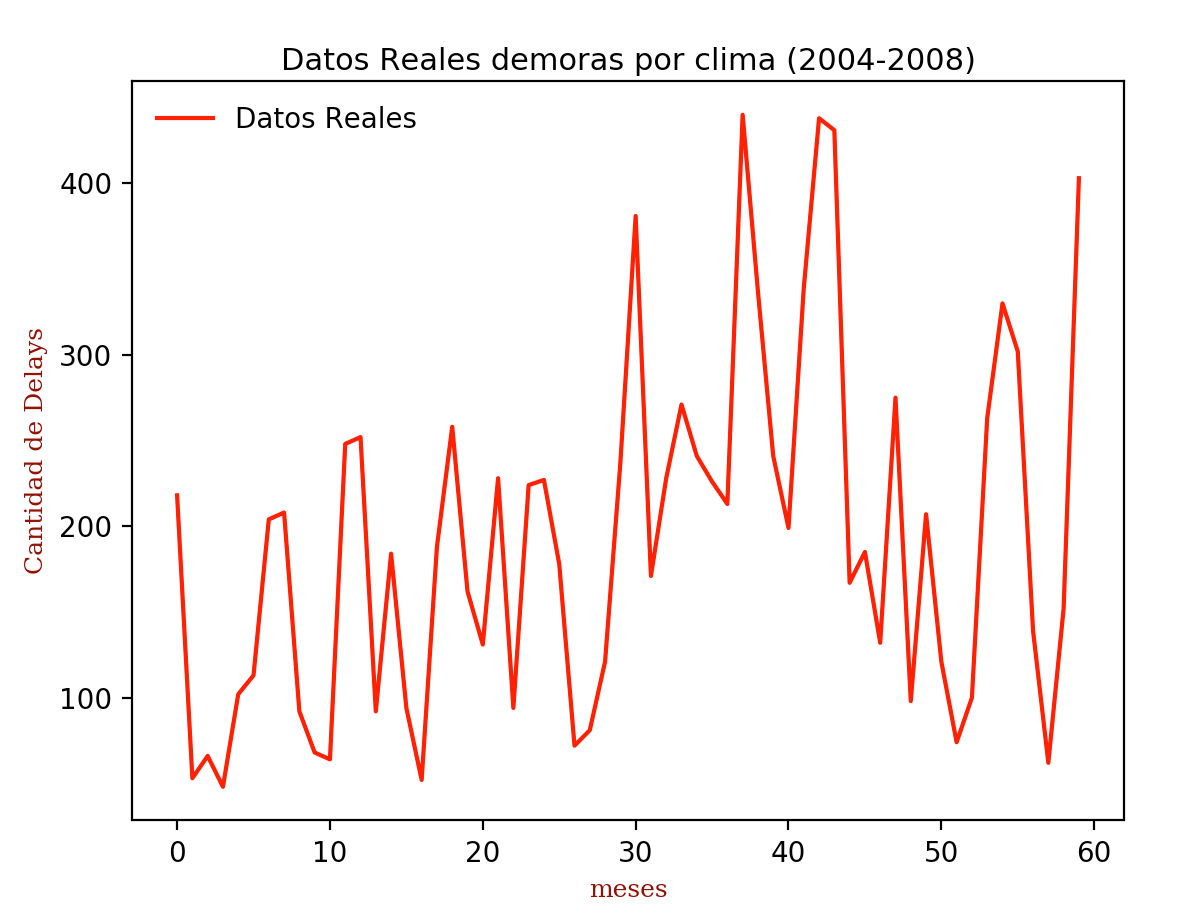
\includegraphics[scale=0.5]{imagenes/reales.png}
\end{center}

Como resultado de esta observaion podriamos decir que las funciones trigonometricas como senos y cosenos podrian sernos de gran ayuda, ademas de que sabemos que las funciones polinomicas pueden aproximar bastante bien.

Por lo que en la experimentacion intentaremos buscar la mejor forma de aproximaci\'on es una combinaci\'on de funciones trigonom\'etricas sobre prolinomios, en la siguiente subseccion pasamos a mostrar el detalle de como llegamos a esta conclusi\'on.

\subsection{Resultados}
En primer lugar tomamos un polinomio de grado impar ($a*x^5+b*x^4+c*x^3+d*x^2+e*x+f$ , siendo $a,b,c,d,e,f$ valores que nos da cuadrados minimos y x el numero de) , ya que luego de comparar contra uno de grado par notamos que era mas suave y tomaba mejor los puntos, para la aproximaci\'on de los meses 0-47, osea los años 2004-2007, con el fin de ver como resultaba la misma arrojando los primeros resultados.

	\begin{center}
	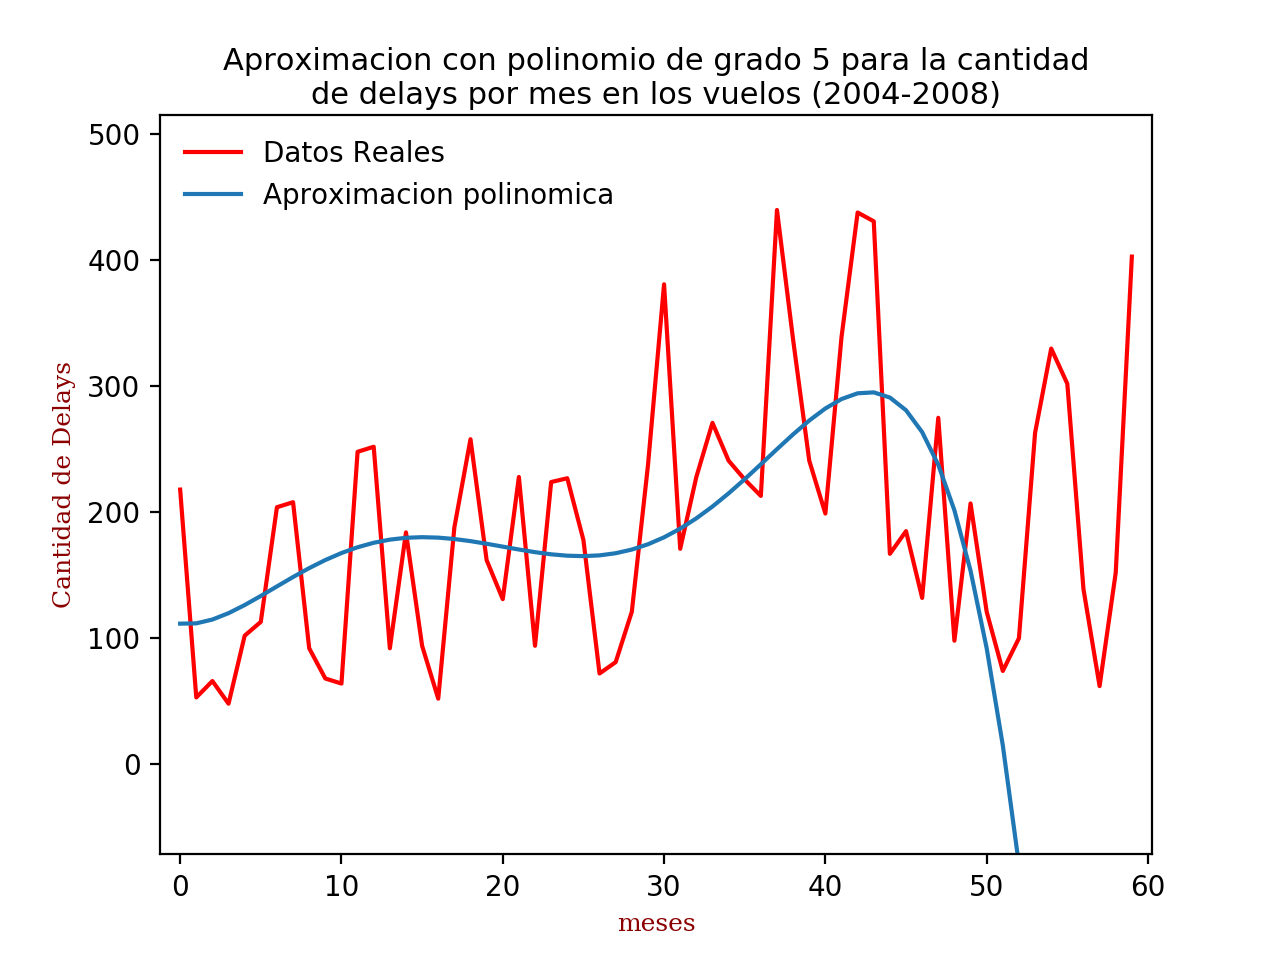
\includegraphics[scale=0.7]{imagenes/delaysPolinomio.png}
	\end{center}

Como podemos ver en el grafico anterior esta aproximaci\'on es buena dentro de los meses de entrenamiento pero el problema que surge es que luego en la aproximaci\'on no aproxima bien haciendo que la funci\'on tienda a menos infinito, siendo este un problema para los polinomios, ya que a lo sumo un polinomio de grado n tiene n derivadas esto nos indica que a partir de un punto va a tender a m\'as o  menos infinito, pero por otro lado el problema es que no podemos agarrar los picos que tiene la funcio\'on real.

Para evitar este problema intentamos aproximar mediante funciones trigonom\'etricas, mas puntualmente con senos y cosenos ya que estas están acotadas tanto superior como inferiormente, la funcion utilizada fue $a*sin(x)+ b*cos(x)+c*sin(2*x)+ d*sin(3*x)+ e*cos(2*x)+f$.

	\begin{center}
	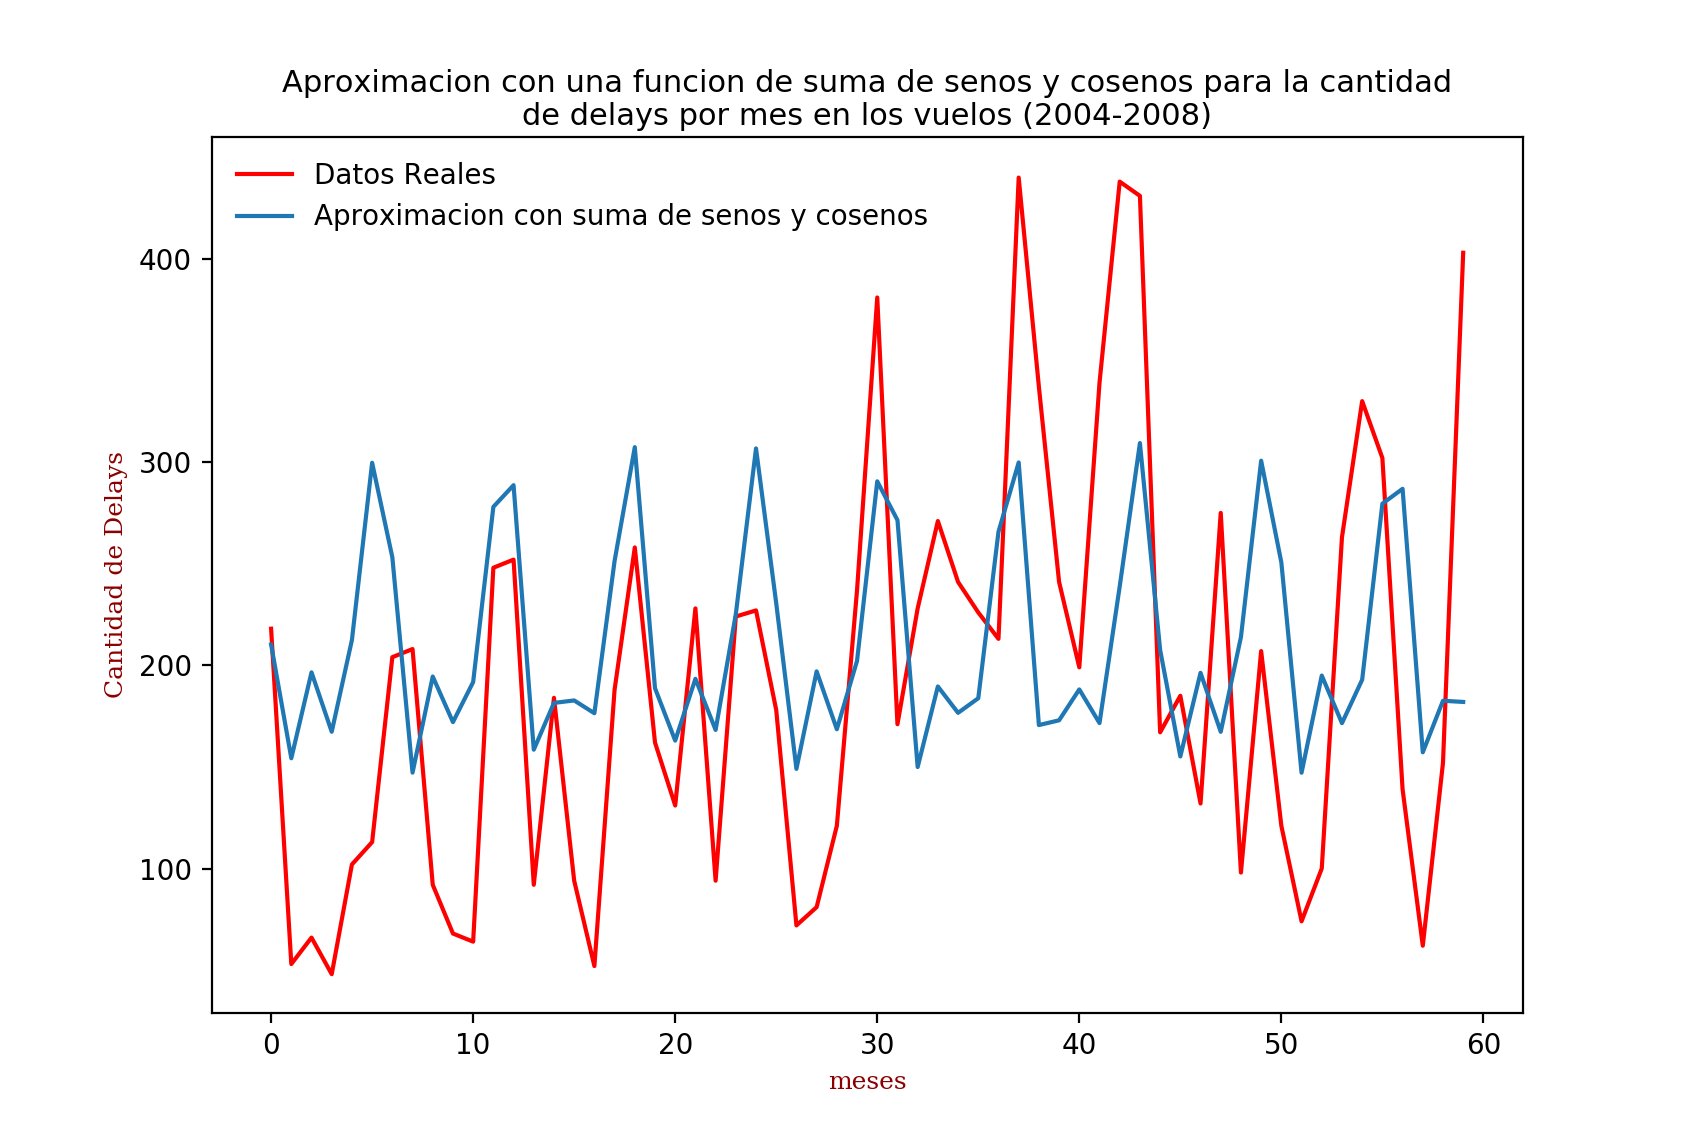
\includegraphics[scale=0.6]{imagenes/senosCosenos.png}
	\end{center}

Como se puede ver en el siguiente gr\'afico, el problema de utilizar estas funciones es que se mantienen dentro de esas cotas en l\'inea recta, con lo cual si nuestra funci\'on a aproximar crece levemente durante toda su grafica no vamos a poder aproximarla bien.
Por lo tanto decidimos hacer una combinaci\'on de ambas funciones para poder aprovechar ambas necesidades que ten\'iamos, que la misma no tienda a infinito luego de los meses de entrenamiento y que en cierta forma podamos captar los picos de la funci\'on a aproximar, con lo que tuvimos una mejor aproximaci\'on.

	\begin{center}
	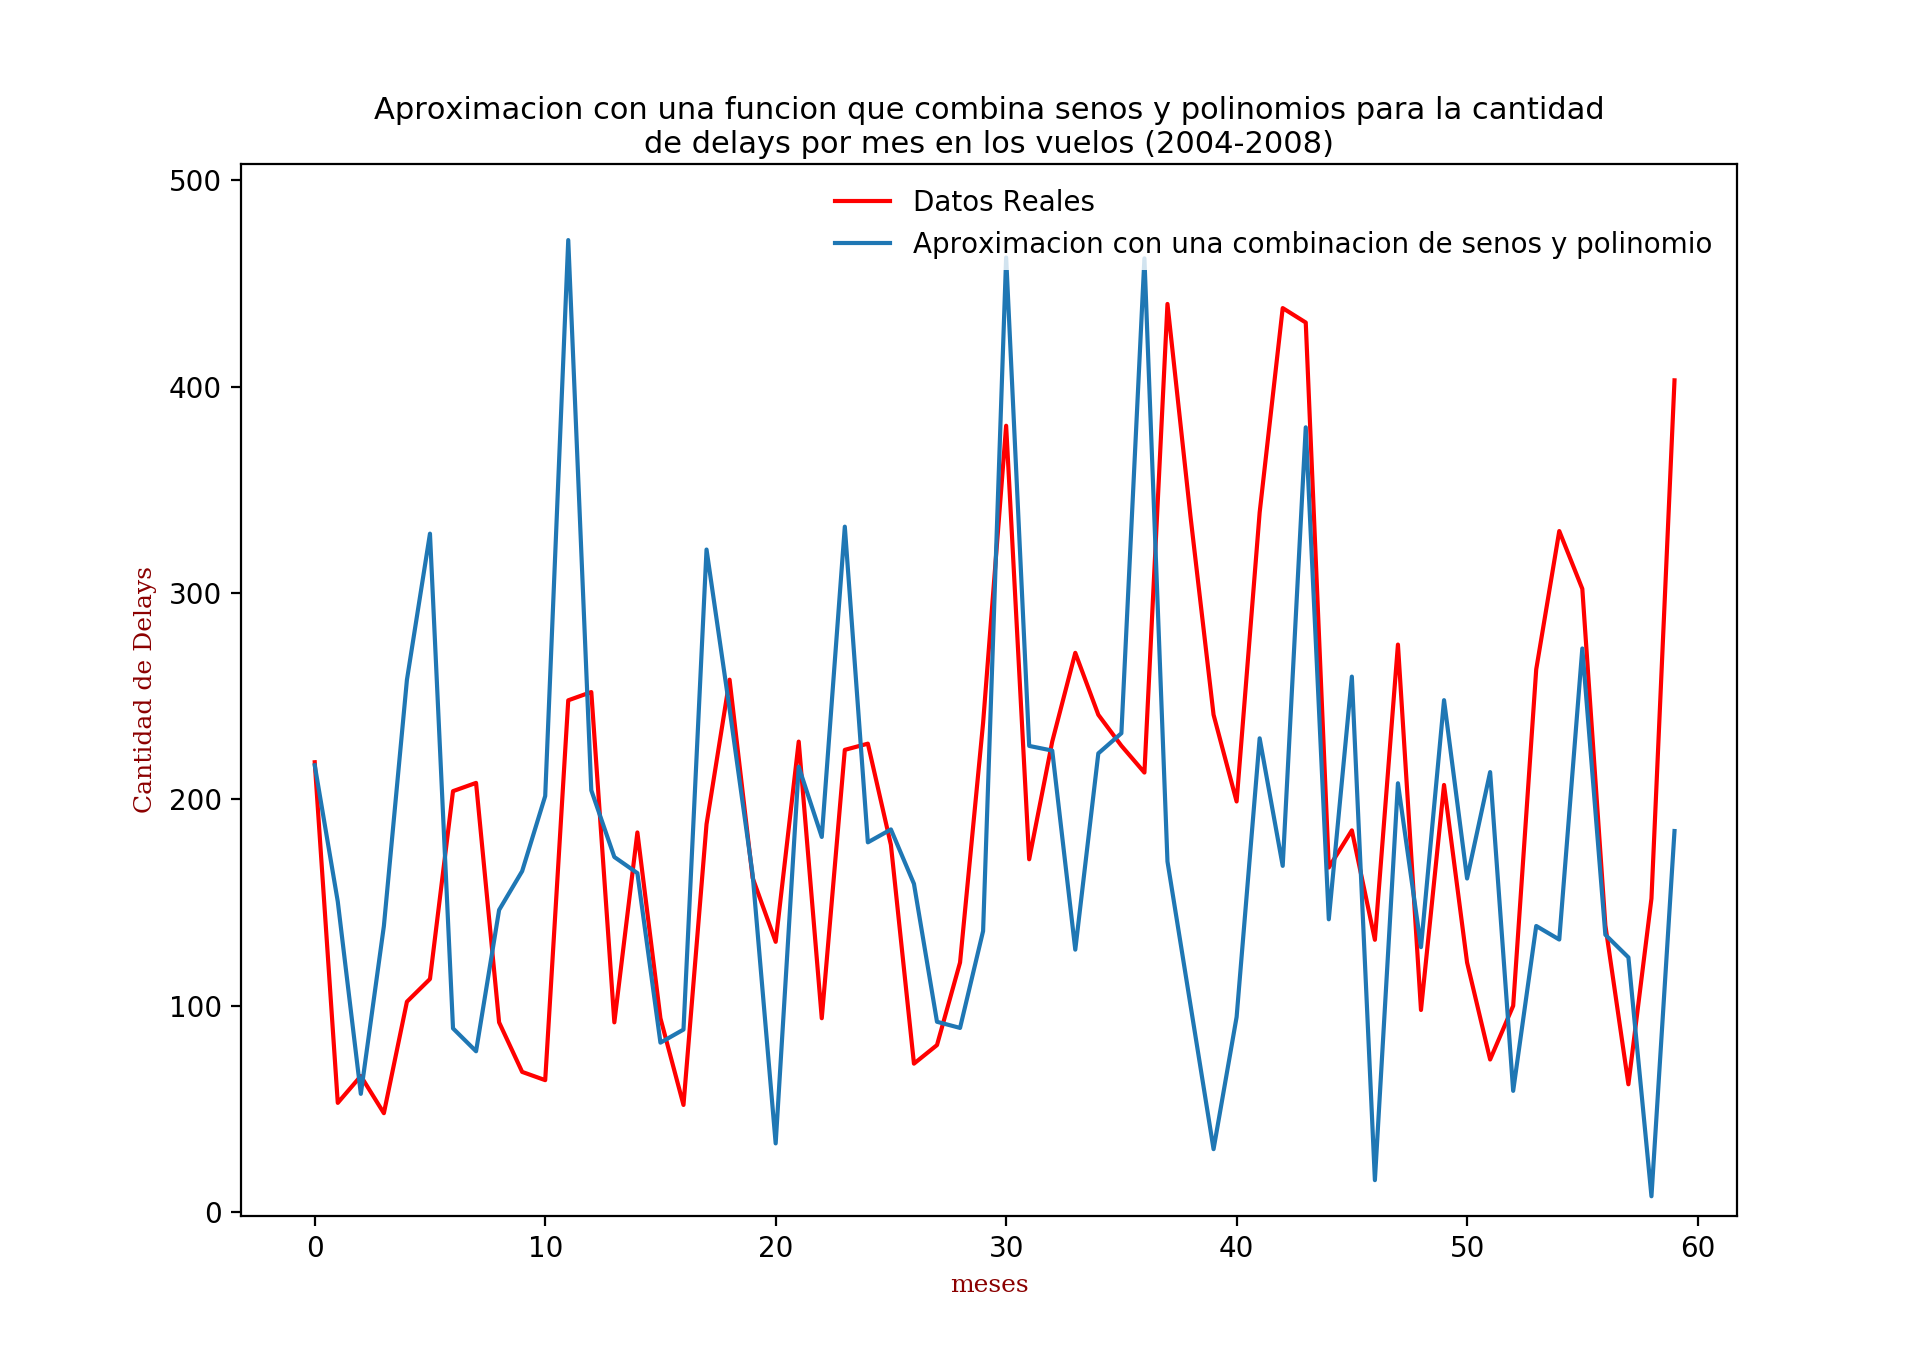
\includegraphics[scale=0.5]{imagenes/polinomioysenos.png}
	\end{center}

Si vemos m\'as en detalle lo que es la aproximaci\'on para 2008 notamos que no tenemos tanto margen de error resultando una buena aproximaci\'on.

	\begin{center}
	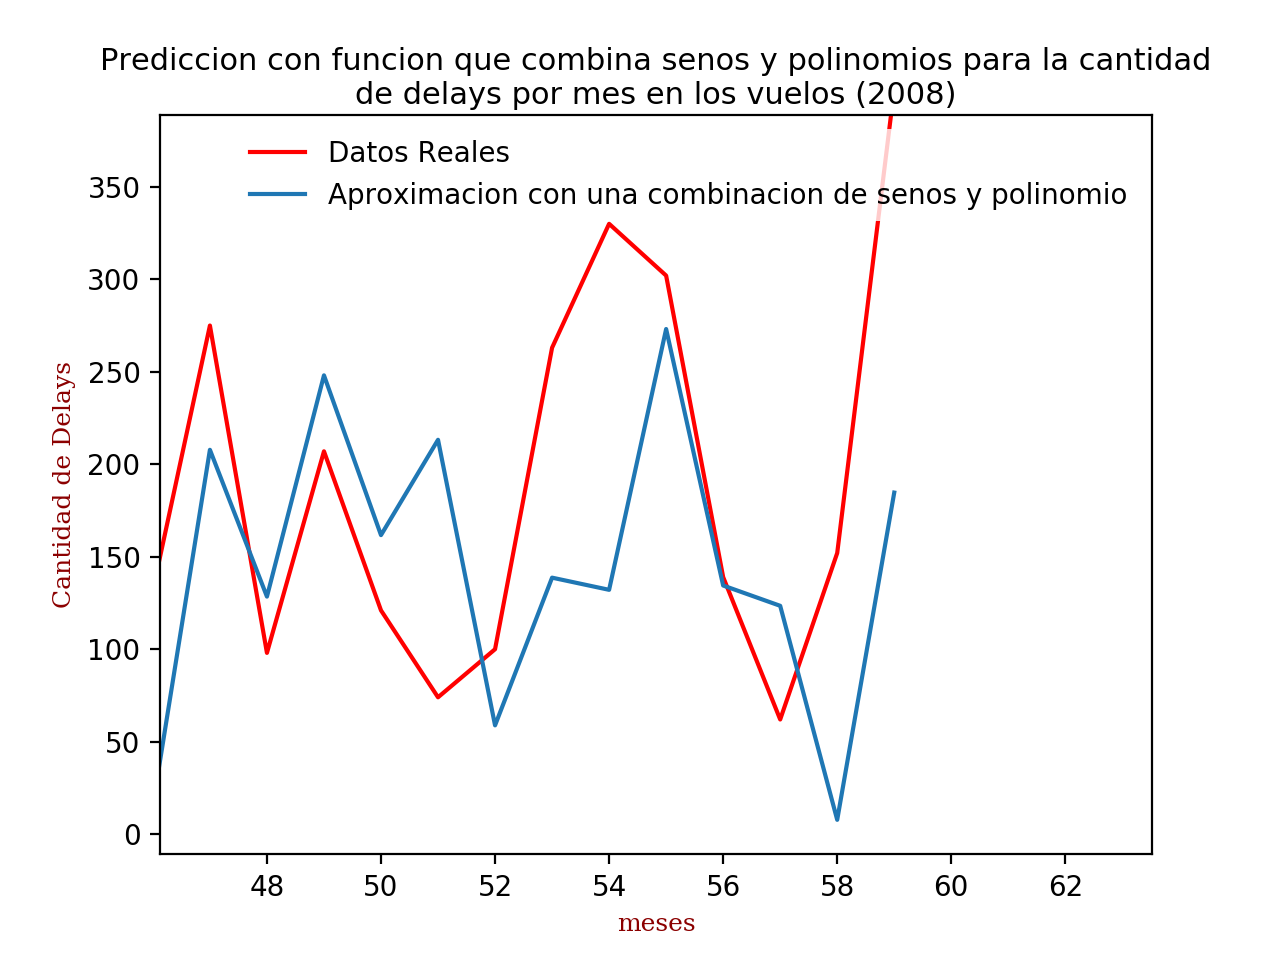
\includegraphics[scale=0.8]{imagenes/delays2008.png}
	\end{center}

Resultando dicha funci\'on $a*sin(x)^5+b*sin(x^2)^4+c*sin(x^2)^3+d*sin(x^2)^2+e*sin(x^2)+f$ y la combinacion de 20 ejecuciones para el cross validation y 24 meses de training.

\section{Comparaci\'on entre vuelos de Delta - American Airlines}

Luego de analizar los datos de vuelo reales de las empresas, comenzamos con la b\'usqueda de funciones que nos permitan predecir de forma relativamente certera los valores reales.

Como en el caso anterior empezamos probando con funciones polin\'omicas, y con el mismo resultado observamos que para obtener predicciones mejores requeriamos una combinaci\'on de funciones trigonom\'etricas y polin\'omincas.

Para la construcci\'on de nuestra predicci\'on tomamos como set de entrenamiento los a\~nos 2004-2007 y realizamos una proyecci\'on sobre el a\~no 2008 comparando los datos reales con la proyecci\'on obtenida por nuestra funci\'on.

En el caso de la empresa \textit{American Airlines} la funci\'on que hacia mejor fit sobre el set de datos fue la dada por:
$a * sen(mes)^5 + b * sen(mes^2)^4 + c * sen(mes^2)^3 + d * sen(mes^2)^2 + e * mes + f$

Presentamos los resultados obtenidos para la proyecci\'on del 2008 en el siguiente gr\'afico

\begin{center}
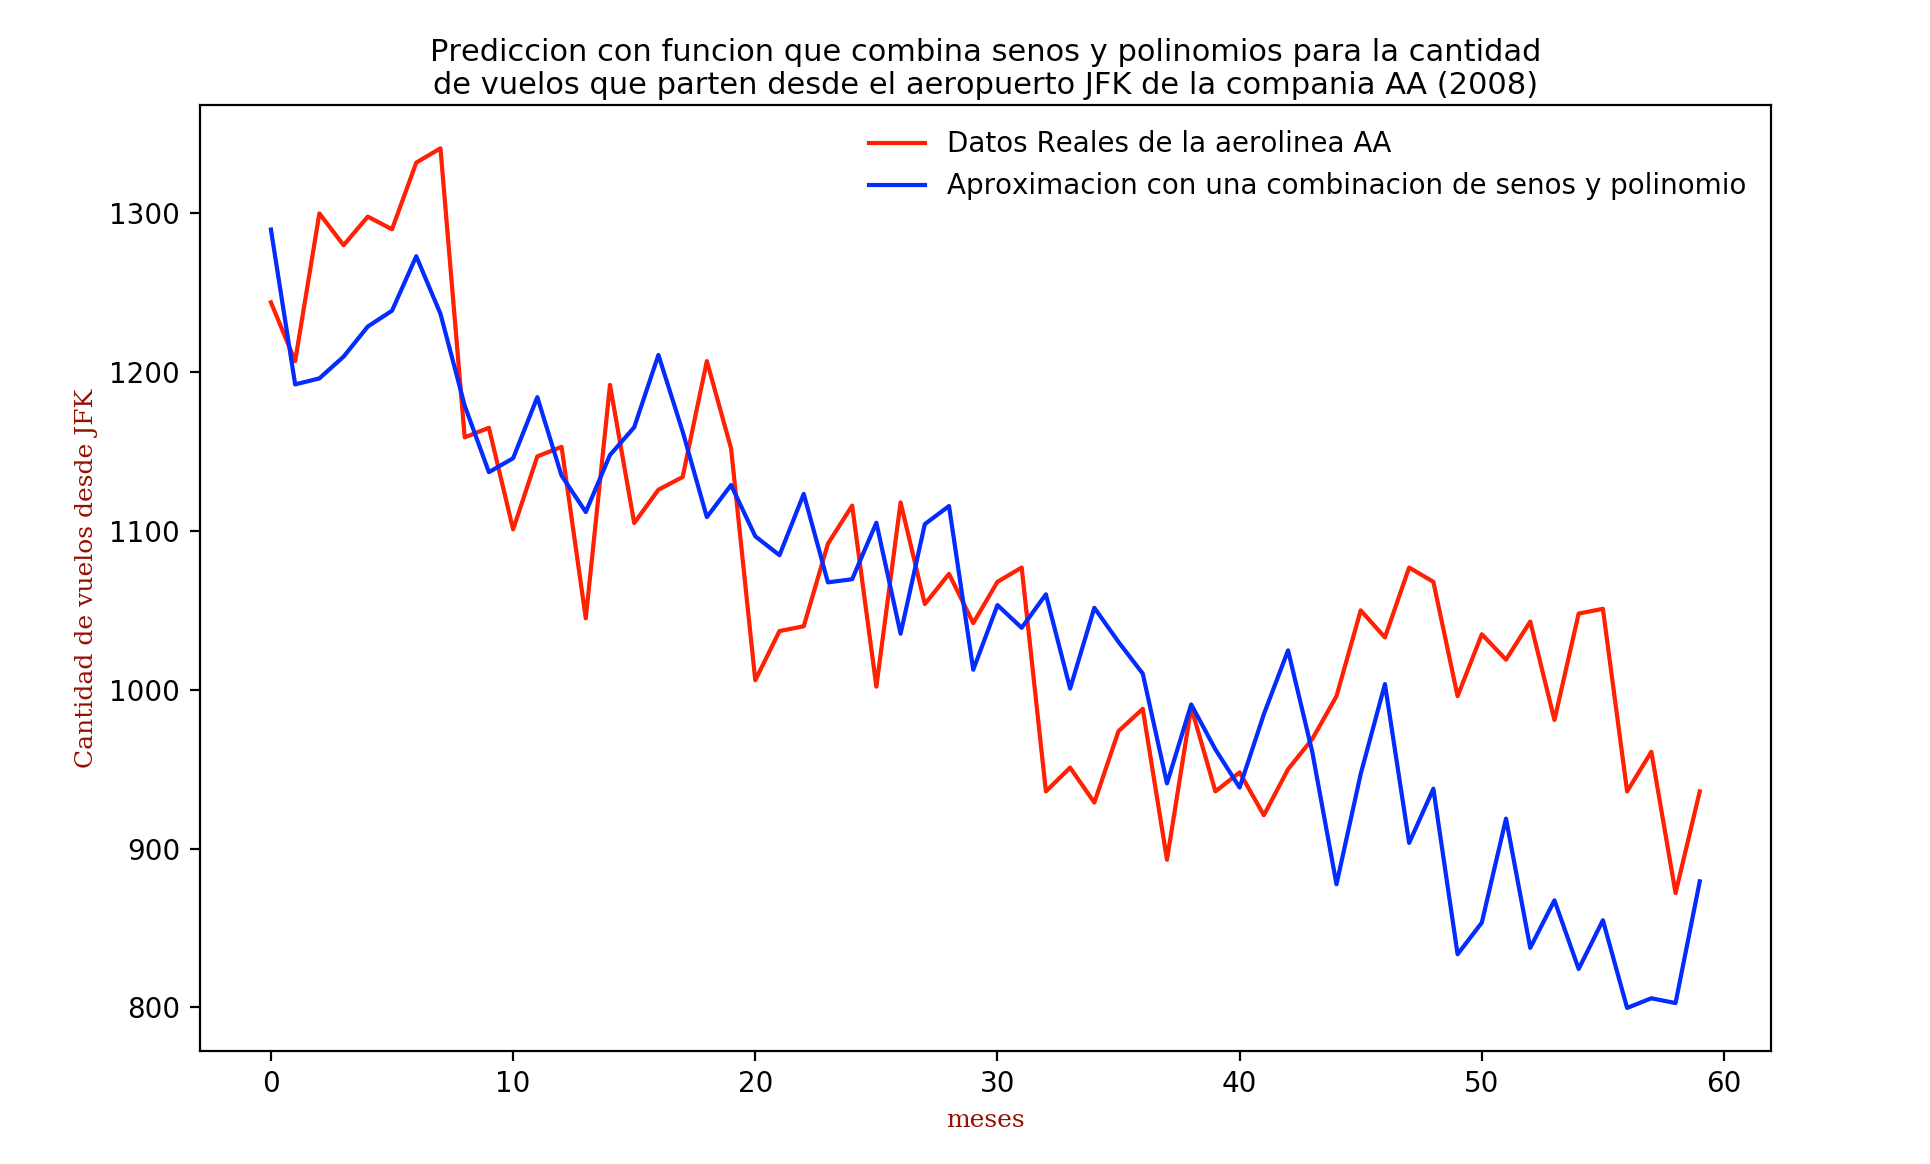
\includegraphics[scale=0.4]{imagenes/AA.png}
\end{center}

En el gr\'afico se puede observar que la funci\'on elegida se comporto de forma similar a la funcion dada por los valores reales, pero de forma mas suave. Es decir, la funci\'on propuesta no es sensible a los valores outliers que se pueden dar por picos de baja o alta demanda, por lo que en meses promedios acompa\~nara la pendiente de los datos reales, pero en mese excepcionales quedara desfazada para ir reacomodandose en el correr del tiempo.

Y para el caso de la empresa \textit{Delta} la funci\'on que hacia mejor fit sobre el set de datos fue la dada por:
$a * tan(mes^6)^4 + b * sen(mes^8) + c * sen(mes^2) + d * sen(mes) +  e$


\begin{center}
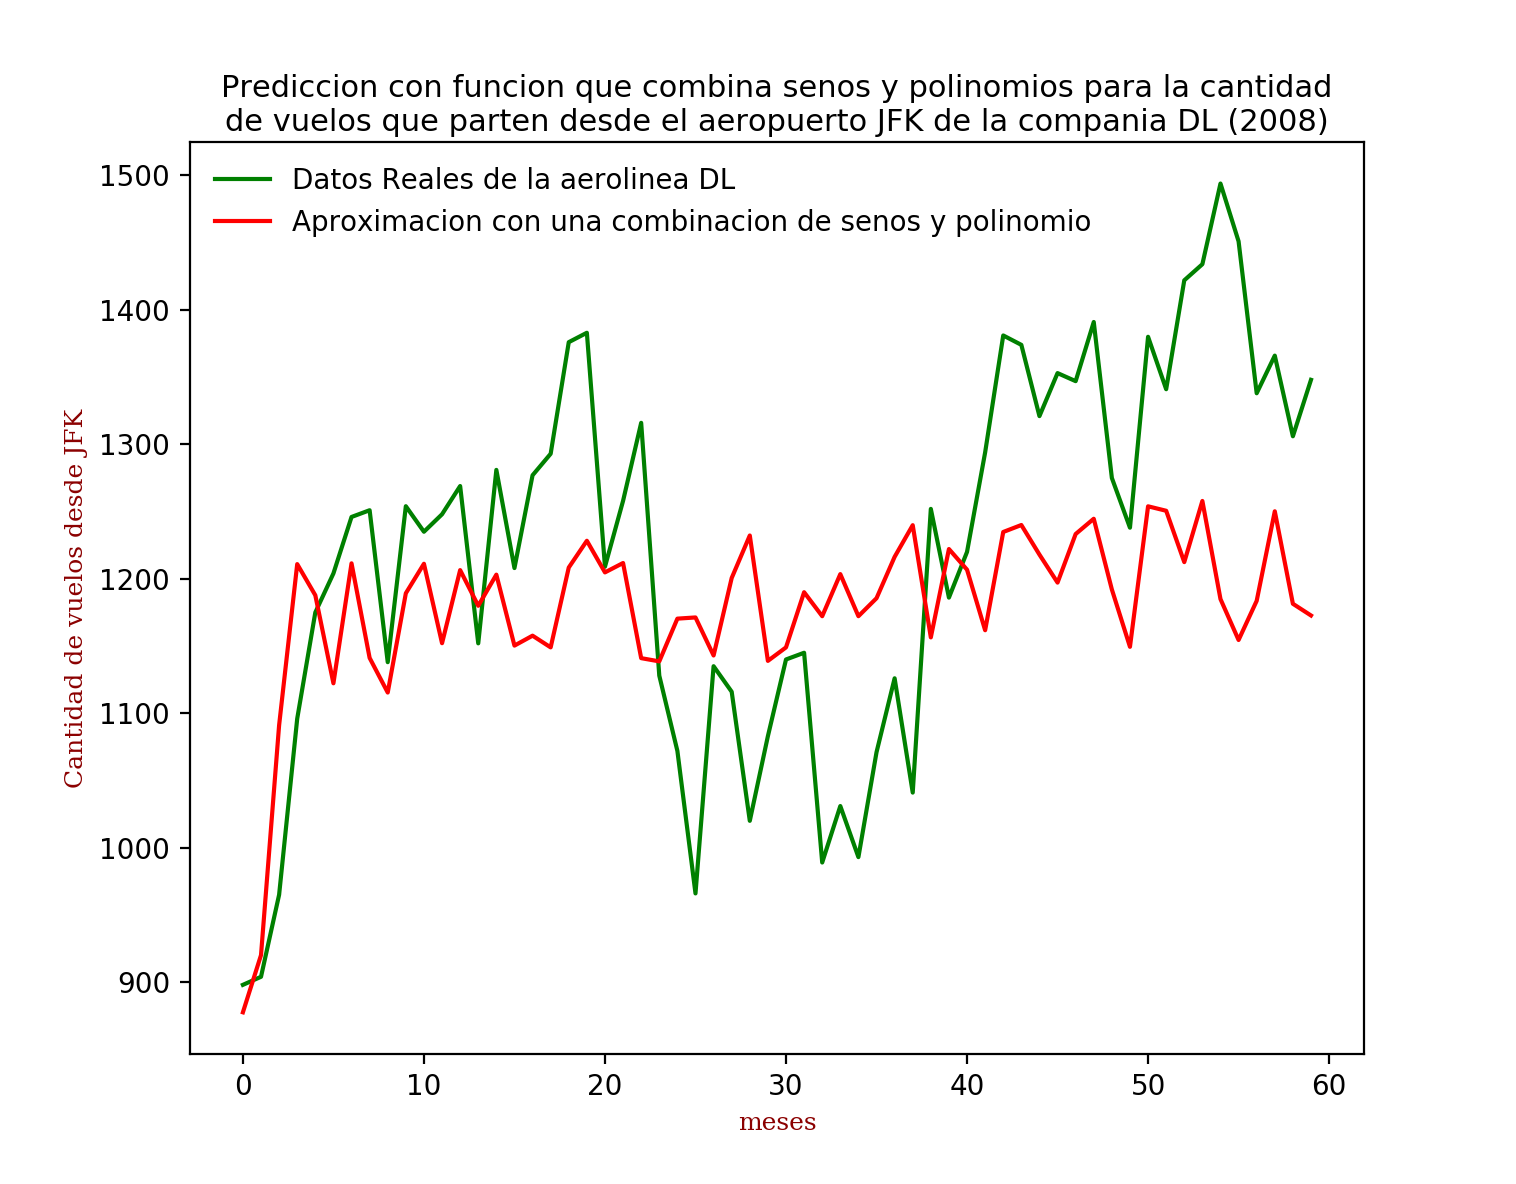
\includegraphics[scale=0.6]{imagenes/DL.png}
\end{center}

En este gr\'afico se puede observar mas el efecto de haber tomado el la funci\'on seno en varios de los coeficientes. Los saltos en la venta de pasajes son suavizados pero siguiendo la misma tendencia. Tomamos la tangente para el coeficiente asociado al $x_0$ porque nos permit\'ia poder representar mejor el crecimiento de de los primeros meses, sin usar una funci\'on exponencial, que en el largo plazo ser\'ia contraproducente ya que el creciemiento de ventas exponencial nunca podr\'ia ser sostenido.



\section{Conclusiones}
	%Hablar sobre la funcion final que escogimos y como reune los que queremos de la dos funciones




\begin{thebibliography}{10}\label{bibliography}
  
\bibitem{bf} Burden, R. L., and J. D. Faires, ``An\'alisis num\'erico,
'' Math. Surveys \textbf{7}, Amer. Math. Soc.,
  Providence, R.I., 1961.
  
\bibitem{d} ASA Section on Statistical Computing. 2009 data expor competition, URL:
  \href{http://stat-computing.org/dataexpo/2009/the-data.html}
  {\texttt{http://stat-computing.org/dataexpo/2009/the-data.html}}.

\end{thebibliography}

\end{document}
